% Figure source for proposal Figure 1:
% "Five-stage pipeline for identifying deception-associated SAE features and performing causal ablation."
%
% Compile standalone with: pdflatex figure_source.tex
% Or extract and paste the tikzpicture block directly into proposal.tex (already done there).

\documentclass[tikz,border=4pt]{standalone}
\usepackage{tikz}
\usetikzlibrary{arrows.meta,positioning}

\begin{document}
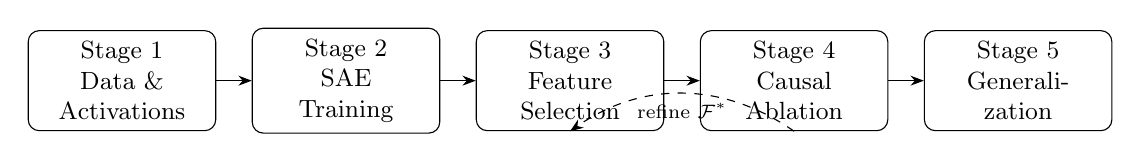
\begin{tikzpicture}[
  node distance=0.55cm and 0.45cm,
  box/.style={draw, rounded corners, text width=2.1cm, align=center,
              font=\small, inner sep=4pt, minimum height=1.0cm},
  >=Stealth
]
\node[box] (data)   {Stage 1\\Data \&\\Activations};
\node[box, right=of data]   (sae)    {Stage 2\\SAE\\Training};
\node[box, right=of sae]    (select) {Stage 3\\Feature\\Selection};
\node[box, right=of select] (ablate) {Stage 4\\Causal\\Ablation};
\node[box, right=of ablate] (gen)    {Stage 5\\Generali-\\zation};
\draw[->] (data)   -- (sae);
\draw[->] (sae)    -- (select);
\draw[->] (select) -- (ablate);
\draw[->] (ablate) -- (gen);
\draw[->, dashed, bend right=35] (ablate.south) to node[below,font=\scriptsize]{refine $\mathcal{F}^*$} (select.south);
\end{tikzpicture}
\end{document}
